% ---------------------------------------------------------------------
% ---------------------------------------------------------------------
% ---------------------------------------------------------------------

\chapter[Sparse N-PLS, a method for variable selection in multiway data sets]{Sparse N-PLS, a method for variable selection in multiway data sets}



% ---------------------------------------------------------------------
% ---------------------------------------------------------------------
\section{Variable selection through L1 penalization}
As explained in \autoref{chapter:modern_techniques}, lasso shrinks all the coefficients of a model, forcing some of them to be exactly zero, effectively performing variable selection by using L1-penalization. Unfortunately the application of lasso, or its generalization elastic net, to three-way or multi-way data is not straightforward. In \autoref{chapter:threeways}, the standard $N$-PLS algorithm has been presented as an appealing technique for modelling three- or multi-way data sets. However, it has been exposed that, although there are some post modelling methods for estimating variable importance such as VIP and selectivity ratio, it does not perform in-model variable selection, which would greatly increase its utility for analyzing metabolomic data. Our approach consists in applying the L1 penalization from lasso inside the $N$-PLS algorithm to be able to perform variable selection at the model-fitting step while maintaining the capability of $N$-PLS of dealing with multi-way arrays. 

For this, we propose using the soft-thresholding operator which can be derived from the lasso problem as follows:

\begin{enumerate}
    \item Assuming \textbf{X} (matrizied version of \textbf{\underline{X}} is composed of orthogonal columns, the least squares solution is
    
    \begin{equation}
        \hat{\beta}^{LS}=(X^TX)^{-1}X^Ty=X^Ty
    \end{equation}
    \item Using the Lagrangian form, an equivalent problem to that considered would be
    
    \begin{equation}
        \min_\beta\frac{1}{2}||y-X\beta||^2_2+\lambda||\beta||_1
    \end{equation}
    \item Expansion of the first term gives
    
    \begin{equation}
        \frac{1}{2}y^Ty-y^TX\beta+\frac{1}{2}\beta^T\beta
    \end{equation}
    Since $y^Ty$ does not contain any of the variables of interest, it can be discarded, and we can consider the following equivalent problem
    
    \begin{equation}
        \min_\beta(-y^TX\beta+\frac{1}{2}||\beta||_2)+\lambda||\beta||_1
    \end{equation}
    Which can be rewritten as
    
    \begin{equation}
        \min_\beta \sum_{j=1}^{p}-\hat{\beta}^{LS}_j\beta_j+\frac{1}{2}\beta^2_j+\lambda|\beta_j|
    \end{equation}
    So, we have a sum of objectives as the objective function. Since each of them corresponds to a separate $\beta_j$, this means that each variable may be solved individually.
    \item For a certain $j$, we want to minimize
    
    \begin{equation}
        \mathcal{L}_j = -\hat{\beta}^{LS}_j\beta_j+\frac{1}{2}\beta^2_j+\lambda|\beta_j|
    \end{equation}
    If $\hat{\beta}^{LS}_j > 0$, then $\beta_j \geq 0$, otherwise we could just change its sign and get a lower value for the objective function. Correspondingly, if $\hat{\beta}^{LS}_j < 0$, then $\beta_j \leq 0$
    \item In the first case, if $\hat{\beta}^{LS}_j > 0$ and $\beta_j \geq 0$, then
    
    \begin{equation}
        \mathcal{L}_j = -\hat{\beta}^{LS}_j\beta_j+\frac{1}{2}\beta^2_j+\lambda\beta_j
    \end{equation}
    After differentiating respect to $\beta_j$ amd setting equal to zero, we get $\beta_j = \hat{\beta}^{LS}_j-\lambda$. Since $\beta_j \geq 0$, the right-hand side must be non-negative, si the solution would be
    
    \begin{equation}
        \beta_j^{lasso}=sgn(\beta_j^{LS})(|\beta_j^{LS}|-\lambda)^+
    \end{equation}
    Which is the soft-thresholding operator.
    \item In the other case, if $\hat{\beta}^{LS}_j < 0$ and $\beta_j \leq 0$, then
    
    \begin{equation}
        \mathcal{L}_j = -\hat{\beta}^{LS}_j\beta_j+\frac{1}{2}\beta^2_j-\lambda\beta_j
    \end{equation}
    After differentiating respect to $\beta_j$ and setting equal to zero, we get $\beta_j = \hat{\beta}^{LS}_j+\lambda$. Since we need $\beta_j \leq 0$ the solution is
    
    \begin{equation}
        \beta_j^{lasso}=sgn(\beta_j^{LS})(|\beta_j^{LS}|-\lambda)^+
    \end{equation}
    Which, again, gives the soft-thresholding operator.
\end{enumerate}

\vspace{20pt}
The soft-thresholding operator is well known in signal processing and image analysis, since it is used as a denoising filter in noisy images to obtain an approximation of the original image which gives the minimum mean square error \parencite{khare2005soft, joy2013denoising}. To understand how it works, the soft-thresholding function for a threshold of 3 has been represented in \autoref{figura28}.

\begin{figure}[hbtp]
\centering
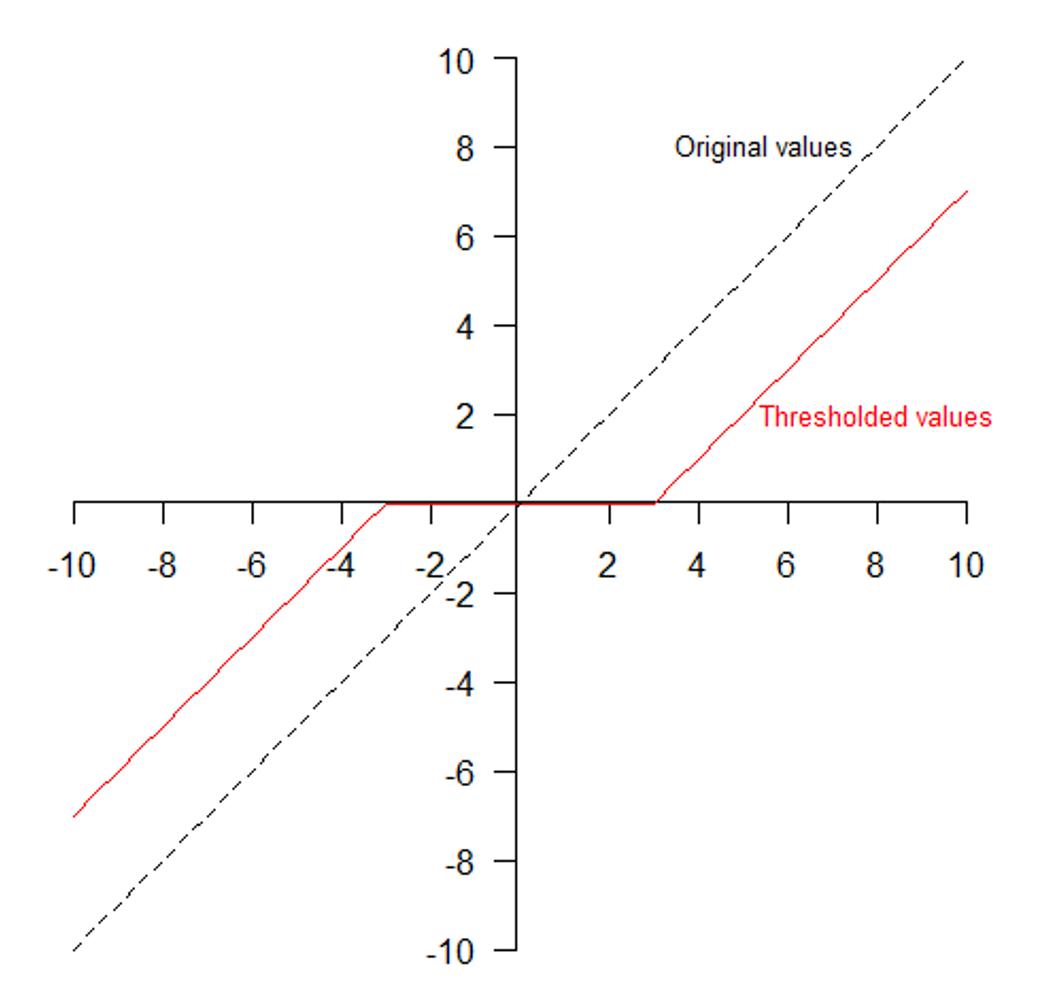
\includegraphics[width=0.6\textwidth]{figura28.png}
\caption{Soft-thresholding function with a threshold of 3. Values higher than the threshold have the threshold value substracted and values equal or less than the threshold are set to zero.}
\label{figura28}
\end{figure}

\section{Sparse N-PLS, integration of L1 penalization in the N-PLS algorithm}
\label{NPLSpenalization}
As commented above, we propose to introduce the L1-penalization in the N-PLS algorithm. To this aim, we used a similar approach to that of \cite{le2008sparse}. Briefly, to achieve sparse versions of $\textbf{\text{w}}^\text{J}$ and $\textbf{\text{w}}^\text{K}$ for each latent variable, we introduce the soft-thresholding penalty function $\beta_j^{lasso}=sgn(\beta_j^{LS})(|\beta_j^{LS}|-\lambda)^+$  in the $N$-PLS algorithm right after the SVD at the $\textbf{\text{w}}^\text{J}$ and $\textbf{\text{w}}^\text{K}$ determination. The complete algorithm is as follows:


\vspace{20pt}
Center \textbf{\underline{X}} and \textbf{\underline{Y}}, and unfold \textbf{\underline{X}} (and \textbf{\underline{Y}} when necessary) into a two-way matrix.

Let \textbf{u} be some column of \textbf{Y}, and set \textit{f}=1

\begin{enumerate}
    \item $\textbf{\text{w}}^\text{T}=\textbf{\text{u}}^\text{T}\textbf{\text{X}}/\textbf{\text{u}}^\text{T}\textbf{\text{u}}$
    \item Build \textbf{Z} by refolding \textbf{w} according to the modes dimensions
    \item Determine $\textbf{\text{w}}^\text{J}$ and $\textbf{\text{w}}^\text{K}$ by SVD
    \item L1-penalization inclusion
    \begin{enumerate}
        \item Apply soft-thresholding on $\textbf{\text{w}}^\text{J}$: $\beta_j^{lasso}=sgn(\beta_j^{LS})(|\beta_j^{LS}|-\lambda)^+$ 
        \item Apply soft-thresholding on $\textbf{\text{w}}^\text{K}$: $\beta_j^{lasso}=sgn(\beta_j^{LS})(|\beta_j^{LS}|-\lambda)^+$ 
        \item Input the new \textbf{w} as kronecker($\textbf{\text{w}}^\text{K}, \textbf{\text{w}}^\text{J}$)
    \end{enumerate}
    \item $\textbf{\text{t}}=\textbf{\text{Xw}}/\textbf{\text{w}}^\text{T}\textbf{\text{w}}$
    \item $\textbf{\text{q}}=\textbf{\text{Y}}^\text{T}\textbf{\text{t}}/\text{norm}(\textbf{\text{Y}}^\text{T}\textbf{\text{t}})$
    \item $\textbf{u}=\textbf{Yq}$
    \item Check for convergence. If it is achieved, continue; otherwise, go to 1
    \item $\textbf{\text{b}} = (\textbf{\text{T}}^\text{T}\textbf{\text{T}})^{-1}\textbf{\text{T}}^\text{T}\textbf{\text{u}} \text{; where} \ \textbf{\text{T}}=[\text{t1}\ \text{t2} \text{…} \text{t}_f]$
    \item $\textbf{\text{X}} = \textbf{\text{X}}-\textbf{\text{tw}}^\text{T} \ \text{and} \ \textbf{\text{Y}} = \textbf{\text{Y}}-\textbf{\text{tbq}}^\text{T}$
    \item \textit{f} = \textit{f}+1. Continue from step 1 until a good description of \textbf{Y}
\end{enumerate}
\vspace{20pt}

This algorithm is applicable to both the standard regression (continuous response) and the discriminant version of the $N$-PLS model, i.e. $N$-PLS-DA. In the case of $N$-PLS-DA, \textbf{\underline{Y}} is a \textbf{y} vector formed by ones and zeros, each of the two values related to one of the two classes to be segregated. 



\section{Parameters of the sparse N-PLS algorithm}
\subsection{Tuning of the parameters}